\documentclass[12pt, twocolumn]{article}

\usepackage[a4paper, hmargin=0.5in, vmargin={0.5in, 1in}]{geometry}
% \usepackage{fullpage}
\usepackage{amsmath,amssymb}
\usepackage{soul}
\usepackage{bussproofs}
% \usepackage{qtree}
\usepackage{graphicx}
\usepackage{dsfont}
\usepackage{multicol}
\usepackage{hyperref}
\usepackage{listings}
\usepackage{mathtools}

\makeatletter
\newcommand*\wrapletters[1]{\wr@pletters#1\@nil}
\def\wr@pletters#1#2\@nil{#1\allowbreak\if&#2&\else\wr@pletters#2\@nil\fi}
\makeatother

% \hypersetup{
%     colorlinks=true,
%     linkcolor=blue,
%     filecolor=magenta,      
%     urlcolor=blue
% }

\title{Cloth Simulation mod for Minecraft}
\author{Samantha Sussman-Randall}

\begin{document}

\maketitle

\section{Outline}

The goal of this project is to create a mod adding cloth simulations to the video game Minecraft \cite{mc}\\

The plan is to create a general framework for running cloth simulations in-game that other mods can make use of, but I plan on adding in some demos along the way as well. Some of the main expected challenges are:
\begin{enumerate}
    \item Getting it to run in realtime with minimal lag.
    \item Allowing it to interact with the game world.
    \item Creating a flexible system that can handle different scenarios (ie different shapes attached to characters, world positions, etc).
    \item Matching the game's style.
\end{enumerate}

\section{Previous Work}

We'll be looking at mass-spring cloth simulations here since it's simpler, but a lot of more recent work in cloth simulations seems to be in neural nets/ML, running on the GPU, or otherwise more niche. We'll also look at some of the previous work specific to Minecraft, mostly to reference style.

\subsection{Previous Cloth Simulation Methods}

We covered some earlier works in class starting with Provot \cite{provot} introducing the mass-spring model with constraints to prevent over-stretching. We also read Baraff \& Witkin's Large Steps in Cloth Simulation \cite{largesteps} where they implement implicit integration allowing for stable simulation of larger time steps. They also introduce inverse mass matrix modification to constraint individual particles.\\

Desbrun, Schröder, and Barr followed the next year \cite{interanim} with a two step predictor-corrector method that approximates implicit integration without solving a linear system each step and then corrects it similarly to Provot. This method runs faster than Baraff \& Witkin's and they've helpfully included pseudocode for it as well.\\

More recently, a group at Nvidia \cite{smallsteps} had success with running multiple smaller steps rather than one larger step. Their work was not exclusive to cloth and seemed to focus more on correctness rather than efficiency, although it was also efficient. They also include a review of previous work that is much more comprehensive than mine.

\subsection{Minecraft Specific Work}

Let's start with Minecraft itself. The game has two cloth-like bits, capes \cite{mccape} and banners \cite{mcbanner}, but I wouldn't quite call them cloth simulations. The cape is a stiff 1 pixel thick rectangular prism that is attached to the player's shoulders and lags behind the players movement. If the player is running forward it'll fly up slightly, if they are falling it'll fly up a lot, if they turn it'll take a second to turn. The banner is similarly a stiff 1 pixel thick rectangular prism that can be hung from a pole or wall. It has a slight swaying animation but otherwise does not interact with its environment. In general, base Minecraft has very limited collision, mostly just a single bounding box per entity. There tends to be a lot of clipping and it generally looks fine!\\

The only in-game cloth simulation I've found is a part of the Physics mod \cite{physicsmod} by Haubna. We can see in a posted demo \cite{physicsmodcloth} that they added a cloth simulation to the banners, capes, and fishing rods. It's hard to tell from the video but there appears to be some slight instability or artifacting on the banners when the character walks through them, although this could just be the character clipping through. The cloth (cape and banner) is completely thin and seems to have decent resolution, skewing more towards realism than blocky stylization. Unfortunately, the mod is closed source and these features are locked behind the developer's Patreon, so it's unclear how they implemented this, how much is java modding and how much is done with shaders.\\

There is also the cloth simulation done for Falkreon's Scarves mod \cite{scarves}. The scarves are completely thin pieces similar to the physics mod, but use textures from the game so they don't feel too out of place.\\

While I was writing this proposal, a friend, Dryym, posted a wonderful hand-animated model of a character with a dress in a Minecraft style \cite{skirt}. They use just a couple of intersecting rectangular prisms textured only on certain sides to give the appearance of flowing cloth. I think this lower resolution style, with only a few bend points, looks very good, but I'm not sure how well it'd work in a cloth simulation without hand animation.

\begin{figure}[h]
    \begin{center}
        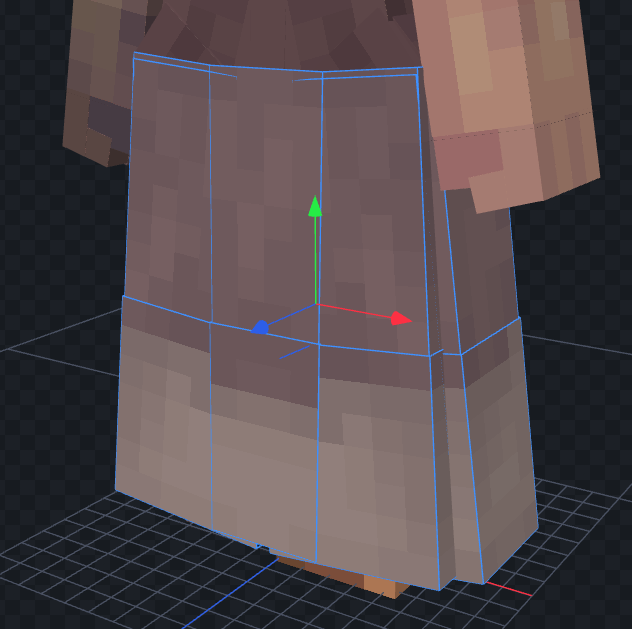
\includegraphics[width=3in]{images/dryym-skirt-blockoutlines-back.png}
    \end{center}
    \caption{Wireframe of Dryym's skirt model}
\end{figure}

\section{The Plan}

I will be following Desbrun's \cite{interanim} work for the cloth simulation, as it seems fast, relatively easy to implement, and has pseudocode included in the paper! For matching style I will be experimenting with lower resolution grids, which should hopefully help with performance, and rendering the cloth with some thickness to match the base game.\\

I will start in a similar place as the physics mod, with modifying the banner and possibly cape renderers to use the cloth simulation. I will then look into collision handling. After that I plan to experiment with the style, work on performance, add an API for easier use of the cloth framework, and/or add other showcases (my heart wants skirts so very badly!)\\

As for a timeline, I'm unfortunately quite behind in the course and this project as of now! I'm also working by myself and don't have a good intuition for how long any of this will take. I'll tentatively say that it'd be good to have something cloth-shaped rendering in-game and most of the code structure setup by midway through the week and have it animating kinda like cloth by next Monday (April 14th). After that, I'll see where the project stands and which of the previously mentioned bits I want to focus on.\\

For mostly irrelevant technical modding details, I'll be modding Minecraft version 1.21.1 supporting the Fabric and NeoForge modloaders using Java 21.\\


\begin{thebibliography}{}
    \bibitem{mc} https://en.wikipedia.org/wiki/Minecraft
    \bibitem{provot} Provot, Xavier. (2001). Deformation Constraints in a Mass-Spring Model to Describe Rigid Cloth Behavior. Graphics Interface. 23(19). 
    \bibitem{largesteps} David Baraff and Andrew Witkin. 1998. Large steps in cloth simulation. In Proceedings of the 25th annual conference on Computer graphics and interactive techniques (SIGGRAPH '98). Association for Computing Machinery, New York, NY, USA, 43-54. https://doi.org/10.1145/280814.280821
    \bibitem{interanim} Mathieu Desbrun, Peter Schröder, and Alan Barr. 1999. Interactive animation of structured deformable objects. In Proceedings of the 1999 conference on Graphics interface '99. Morgan Kaufmann Publishers Inc., San Francisco, CA, USA, 1-8.
    \bibitem{smallsteps} Miles Macklin, Kier Storey, Michelle Lu, Pierre Terdiman, Nuttapong Chentanez, Stefan Jeschke, and Matthias Müller. 2019. Small steps in physics simulation. In Proceedings of the 18th annual ACM SIGGRAPH/Eurographics Symposium on Computer Animation (SCA '19). Association for Computing Machinery, New York, NY, USA, Article 2, 1-7. https://doi.org/10.1145/3309486.3340247
    \bibitem{mccape} https://minecraft.wiki/w/Cape
    \bibitem{mcbanner} https://minecraft.wiki/w/Banner
    \bibitem{physicsmod} https://minecraftphysicsmod.com/
    \bibitem{physicsmodcloth} https://www.youtube.com/watch?v=9eapNwKztkM
    \bibitem{scarves} https://modrinth.com/mod/scarves
    \bibitem{skirt} \wrapletters{https://www.reddit.com/r/Eldenring/comments/1jmo3gg/a\_friend\_of\_mine\_wanted\_a\_custom\_minecraft/}
\end{thebibliography}

\end{document}